\documentclass{article}
\usepackage[utf8]{inputenc}
\usepackage{abstract}
\usepackage{hyperref}
\usepackage{blkarray}
\usepackage{amsmath}
\usepackage{tikz}
\usepackage{array}
\usetikzlibrary{automata}
\usepackage{csquotes}
\usepackage{multirow}

\newcolumntype{P}[1]{>{\centering\arraybackslash}p{#1}}

\title{Machine Learning Project Final Report}
\author{Pablo Bollansée}
\date{May 2016}


\begin{document}

\maketitle

\begin{abstract}
% Motivation
%  - Why do we care?
As the IT world converges to more adaptability, it makes only sense that the web browsers are also trying to adapt themselves to the user in the best possible way.
Therefore, predicting which web page a user wants to visit next could prove to be very interesting.
I try to offer a solution, based on machine learning techniques, to predict the destination web page without going through multiple clicks.

In this paper I propose a combination of a Markov chain to predict the next possible web pages, and using the time spend on pages as an indicator of the interest in a certain page.
I tried to create a system where guessing next pages of interest is fast enough to be used in a real-time application.
\end{abstract}

\section{Introduction}
% wat we precies doen
This section specifies the problems that were addressed with this project, the goals of the project, and some questions I wanted to answer. 

\subsection{Problem description}
We were given a log of all links a user clicks, pages he or she loaded and times-stamps for when these actions happened. 
These are called click streams.
I want to predict possible web pages the user is interested in based on these click streams.
The idea is that many web sites have specific pages that are most interesting to people.
These pages might not be the front page however.
Some will require multiple clicks to reach.
I want to predict which pages are the interesting ones and give direct links to the user.

\subsection{Approach}
% Approach
% - How did you go about solving or making progress on the problem?
% - Did you use simulation, analytic models, prototype construction, or analysis of field data for an actual product? 
To realise my goal, I built a prototype that extracts the data from comma-separated values (CSV) files which consists of click streams of several users.
These files are processes to predict which URLs are more likely to be visited next when a user is active on a specific URL.

% - What important variables did you control, ignore, or measure?
I used a Markov Chain representation which is proven to be an effective way to represent these kinds of streams.
In \cite{davison1998predicting} a Markov chain is iteratively build using logs of UNIX console commands.
Each time a new command is used, the existing model is updated rather than a new model learned from scratch.
In a similar way I tried learning web pages.
Each time a user clicks on a link to go to a new page the Markov chain's weights are updated.
This is done by increasing the weight of the node corresponding to that click, and scaling all other nodes.
In \autoref{fig:example_markov_chain} an example of such a Markov chain is shown.

\begin{figure}
    \centering
    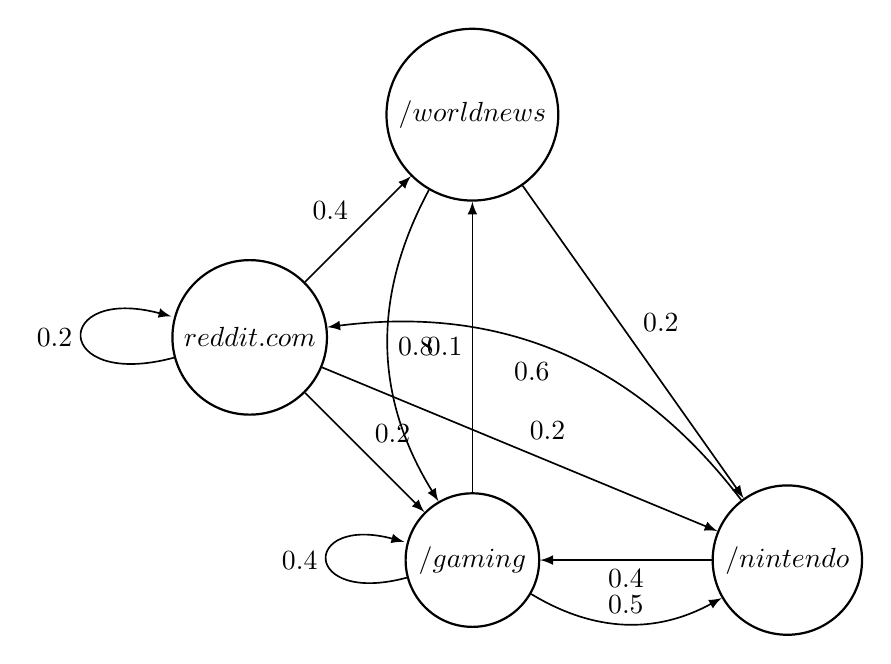
\begin{tikzpicture}[->,>=latex,auto,semithick,node distance=4cm]
    \tikzstyle{every state}=[fill=white,draw=black,thick,text=black,scale=1]
    \node[state]    (reddit)                                {$reddit.com$};
    \node[state]    (worldnews)  [above right of=reddit]    {$/worldnews$};
    \node[state]    (gaming)     [below right of=reddit]    {$/gaming$};
    \node[state]    (nintendo)   [right of=gaming]    {$/nintendo$};
    \path
        (reddit)    edge                node{$0.4$}     (worldnews)
                    edge                node{$0.2$}     (gaming)
                    edge                node{$0.2$}     (nintendo)
                    edge[loop left]     node{$0.2$}     (reddit)
        (worldnews) edge[bend right]    node{$0.8$}     (gaming)
                    edge                node{$0.2$}     (nintendo)
        (gaming)    edge                node{$0.1$}     (worldnews)
                    edge[loop left]    node{$0.4$}     (gaming)
                    edge[bend right]    node{$0.5$}     (nintendo)
        (nintendo)  edge                node{$0.4$}     (gaming)
                    edge[bend right]    node{$0.6$}     (reddit);
    \end{tikzpicture}
    \caption{Example Markov chain for reddit.com}
    \label{fig:example_markov_chain}
\end{figure}

Secondly I will use the time spend on a page as an indication of how interested a user is in a page.
In \cite{gunduz2003web} they found that indeed, time spend on a page is a good indication of the actual interest of the user in that page.
This also makes sense, if a user is only visiting a page to get to another one, he will presumably quickly click on a link, rather than staying on that page.
However if a user really is interested, he will stay on that page to be able to read the content.
Similarly to how I build the Markov chain, this time spend on a page is built up iteratively.
This will make more recent pages to be more important as user's interests might change over time.
However, if their interests don't change, the same weights will continuously be refreshed.

\subsection{Goals and questions}

The main goal of this project is to find an efficient way to predict pages of interest of a user.
I want this method to be able to be used in a real-time application such as a web-browser.

Some questions I wanted to address:

\begin{enumerate}
  \item Can a simple matrix representation of clicks capture the sequence data in an acceptable amount of memory? Even with the derivatives of URLs?
  \item How important are derivative URLs in the final decision?
  \item Can this relatively simple approach give good predictions?
  \item Is my approach fast enough to use in a real-time application?
  \item How well does data from users predict another user?
\end{enumerate}

\section{The Algorithm}

The algorithm is subdivided in two parts: A learner and a guesser.
The learner processes all the csv files, as well as incoming clicks.
The guesser uses the learned information to predict web pages the user might want to visit.
As stated earlier in the report, I want the guesser to be as fast as possible.
To achieve this, the model is made so that virtually all the learning and guessing can be done beforehand.
This leaves very little calculations that need to be done when requesting guesses.

The algorithms allows for learning during the current user-session.
I call this "dynamic learning".
This however means a lot of processing is required during the use of the program, as no heavy optimizations were done in the code.
Disabling the dynamic learning will make it possible to process everything needed before any guesses are done, making the algorithm very fast, but less flexible.

\subsection{Preprocessing}

As my learner builds on a model iteratively, I had to select some order for the click-stream data.
As suggested in \cite{davison1998predicting} and by common sense, more recent entries are more relevant, as user preference might change over time.
I also consider each file to be a single user-session.
So before learning from any log-files, I sorted them based on their starting time.
This was done by simply reading the first entry in each file, and sorting them by those time-stamps.
Empty or unreadable files were discarded.

To read each line in a log file, I assumed a fixed structure and parsed them accordingly.
The lines were simply parsed manually, splitting them on the comma and then parsing each part.
Each line contains a time stamp, a command-type, a URL, and a second URL for $click$-commands.
I used the command of type $load$, $beforeunload$ and $click$.
Command of different types were ignored.

URLs are also cleaned.
This simply means that parameters are removed from them (everything after a "?" is removed) and trailing slashes are removed.

Lastly for each URL one or several derived URLs are created.
For instance, if the data has a load-event for "www.example.com/some/page" the same load event is considered for both "www.example.com/some" and "www.example.com".
The depth of the derivation ("www.example.com/some" has depth 1 and "www.example.com" depth 2) is also given to the learner for considerations.

\subsection{Learner}

The learner processes all information.
This information comes in two parts: the CSV logs, as well as actions done during a user-session if the program is running.
Each line in a log-file and each action done during a user-session is handled in exactly the same way.

Each click-event is used to build the Markov chain of websites that follow each other. The load-and beforeunload-event are used to determine the time spend on a page, thus indicating a user's interest in this page.

\subsubsection{Building the Markov chain}

The first part of the learner is the Markov chain.
As stated above, the click-events are used to build this.
These events contain two URLs: the URL on which the click was performed (the "from-url"), and the URL to which the click will lead us (the "to-url").
The Markov chain is simply represented as a matrix, with the rows representing the from-urls, and each row the to-urls.
Each cell represents the chance of going from one page to the next.
This however is not an exact chance, based on counting or something similar, but is build up iteratively as follows:

\begin{itemize}
    \item First the cell corresponding to this click is increased by a certain amount X
    \item If one or both of the URLs are derived URLs, then X is multiplied by some scaling factor
    \item Then the entire row is scaled so that the sum is 1
\end{itemize}

If any URL has never been seem before, a new row and column for that URL are created first, containing only 0s.

The matrix, for the example in \autoref{fig:example_markov_chain} is as follows:

\[
\begin{blockarray}{ccccc}
& reddit.com & /worldnews & /gaming & /nintendo \\
\begin{block}{c(cccc)}
    reddit.com      & 0.2           & 0.4           & 0.2       & 0.2 \\
    /worldnews      & 0             & 0             & 0.8       & 0.2 \\
    /gaming         & 0             & 0.1           & 0.4       & 0.5 \\
    /nintendo       & 0.6           & 0             & 0.4       & 0   \\
\end{block}
\end{blockarray}
\]

\subsubsection{Remembering time}

The second part of the learning consists of remembering the time spend on a page.
This is done by iteratively building a list witch represents an indication of the time spend on each page.
This list uses the same indexes as the Markov chain matrix.

Again this list is build up iteratively.
Each time a new url is loaded the time-stamp is remembered, then when a url is unloaded the time spend on that page is added to the corresponding item in the list.
This list then represents to total time spend on a page.
To prioritize urls visited more recently, a scaling factor is applied to the entire list before adding the new time.
Urls that are only visited very occasionally will be scaled down many time, thus their importance is decreased, while urls visited very often will build up importance over time.

An example time vector would be:
\[
\begin{blockarray}{cccc}
reddit.com & /r/worldnews & /r/gaming & /r/nintendo \\
\begin{block}{(cccc)}
    1 hour & 15 minutes & 20 minutes & 10 minutes \\
\end{block}
\end{blockarray}
\]

\subsection{Guesser}

The guesser uses all information build up during learning.
This is done in such a way that it only has to happen once each time the learned data is updated.
So the guesser only has to be updated once after learning, and can then guess for any url it knows.
Very little calculations will need to be done when requesting guesses for a certain url, making the algorithm very fast.
However, this only works when the learner isn't updated during a session (disabling "dynamic learning").

The guesser combines all the data from both parts of the learner.
It uses the Markov chain to create possible destination url, and the time-indication to scale the weight these urls get.

The Markov chain created by the learner contains weights that are scaled so that each row has a total weight of 1.
This represent some chance of going from some url to another in \textbf{a single click}.
Since I am trying to predict not just the next url to visit, but urls several clicks in the future this isn't enough.
The guesser therefore builds a combined matrix for multiple clicks.
Let's call the Markov chain matrix $M$, then the combined matrix from the learner is: $M_{total} = M + s^2 M^2 + s^3 M^3 + ...$, with s some scaling factor.
This gives a combined matrix for a single click in the future, two clicks in the future, three clicks, ...
This is a relatively simple idea, but the great thing about it is that it allow the guesser to do this calculation once, and then reuse that same combined matrix for all the guesses.

When guesses for a certain url are requested, the guessed combines the time-spend-on-url vector and one ore more rows from the total matrix $M_{total}$ to create several guesses.
This is done by taking the row for the url and its derivations, scaling them with the times-vector, and adding them together.
To prevent outliers of time spend on a page I borrowed a robust fitting function: $scale * (time^2 / (width^2 + time^2))$, where $scale$ and $width$ are hyperparameters of the algorithm.
This will give a weight to each known url, indicating how likely it is for a person to be interested in that page.
Then the top-X of these urls are returned as guesses.
If the url and all it's derivations are unknown no guesses can be done for it, and nothing is returned.
I chose to return nothing, rather than (for instance) the 5 most visited websites.
This gives a clearer picture of when the guesser is actually working, which seemed more interesting for this prototype.

\section{Experiments}

As stated earlier each log file is considered as a separate user-session.
All tests are done with a user-session as a single entity.
So for each test I divide the user-sessions in some way to get a learn-set and a test-set.
I first let the learner learn from the learn-set.
Then I take each user-session from the test-set and test the predictions as follows:

\begin{enumerate}
    \item Take a load-event from the session
    \item Let the guesser guess for the url of this event
    \item Check the load-events \textit{after} the selected one for urls that were guessed
\end{enumerate}

As I am trying to predict urls several click way, it made no sense to look at the click events.
All web pages that are reached by a click event will also have a load event, so the only information a click event gives is from which page to which the user is going.
This is not relevant for what I am trying to do, as I'm not trying to predict direct clicks, but rather web pages that are several click away.
So I only consider the load-events.

I used two criteria for success:

\begin{enumerate}
    \item If any of the guesses urls were present in the rest of the log
    \item How many of the guessed urls were present in the rest of the log
\end{enumerate}

The first gives a general indication of the accuracy of the model.
While the second gives a more fine-grained look at the guesses, giving a penalty to incorrect guesses.

For instance, if the user is on "www.website.com" and want to go to "www.website.com/some/page" he might go there by first clicking on a link to "some" and then on "page".
The log file will thus show three load-events: "www.website.com", "www.website.com/some", "www.website.com/some/page".
The guesser will thus be asked to guess for "www.website.com".
If the guesser returns "www.website.com/some/page" and "www.website.com/other", this will be counted as a success by the first criteria, as indeed "www.website.com/some/page" was correctly guessed.
However, the second criteria will count this as one succes and one failed guess, since the guesser also returned "www.website.com/other" (assuming it wasn't also visited).

I also tested to see if derived urls are important, by running all tests with derived urls both enabled and disabled in the learner/guesser.
I also changed the tester to consider a guess for a derived url to be correct or not.
For instance, in the above example, if the guesser would guess "www.website.com/some" it could be considered correct because it's a derivative of "www.website.com/some/page".

Using this method of evaluation I created several different test/learn-set combinations:

\subsection{Per-User Cross-validation}

My first experiment is a classic cross-validation test.
I divided each user's log files into 3 random subsets, 2 of which will be learned from, and the remaining one tested on.
I decided on the 2/3 split because many user's only had a few session.
Users with less than three usable sessions were ignored.

\subsection{Per-User Time test}

For each user I divided the sessions up in the 2/3 oldest sessions, and 1/3 newest ones, to test how well older behaviour predicts future trends.
Again users with less than three usable sessions were ignored.

\subsection{Inter-user test}

Next I wanted to see how well users predict the actions of each other.
This was done by dividing all the log files into groups of their corresponding users.
The learner then learns from all but one user, and the remaining user was tested on.

\subsection{Global Tests}

To test how well the method scaled to bigger data sets, I also did a similar cross-validation and time-test, but now with all users combined into one big dataset.
This does not give realistic personalized results of course, as many different users are combined, but allowed me to test on a bigger dataset than each user separately.

\section{Test results and observations}

Here I show the results of my tests.
I show both the macro average (average of the average of each user), and a micro average (average over all data, so users with more data will weigh more heavily).
I also show results for when the learner uses derived urls, and for whether the tester considers derived urls to be correct guesses.

\subsection{Per-User Tests}

As stated before, some users with too little sessions are ignored. These are users 3, 6, 7, 9, 10, 11, 16, 17, 20, 23 and 27.
This leaves 16 of the users that were tested on.

\begin{center}
\begin{tabular}{l |  P{1cm} | P{1.4cm} || P{1.3cm} | P{1.3cm} | P{1.3cm} | P{1.3cm}}
Test & Number of Guesses & Derived learner / tester & Criter-1 macro avg & Criter-2 macro avg & Criter-1 micro avg & Criter-2 micro avg \\ \hline

Cross-val    & \multirow{2}{*}{1} & \multirow{2}{*}{yes / yes} &  0.53 & 0.53 & 0.50 & 0.50 \\
Time         &                    &                            &  0.56 & 0.56 & 0.64 & 0.64 \\ \hline

Cross-val    & \multirow{2}{*}{1} & \multirow{2}{*}{yes / no} &   0.11 & 0.11 & 0.10 & 0.10 \\
Time         &                    &                           &   0.14 & 0.14 & 0.17 & 0.17 \\ \hline

Cross-val    & \multirow{2}{*}{1} & \multirow{2}{*}{no / yes} &   0.18 & 0.18 & 0.17 & 0.17 \\
Time         &                    &                           &   0.21 & 0.21 & 0.19 & 0.19 \\ \hline

Cross-val    & \multirow{2}{*}{1} & \multirow{2}{*}{no / no} &    0.18 & 0.18 & 0.17 & 0.17 \\
Time         &                    &                          &    0.20 & 0.20 & 0.19 & 0.19 \\ \hline \hline



Cross-val    & \multirow{2}{*}{3} & \multirow{2}{*}{yes / yes} &  0.58 & 0.53 & 0.55 & 0.51 \\
Time         &                    &                            &  0.58 & 0.53 & 0.67 & 0.65 \\ \hline

Cross-val    & \multirow{2}{*}{3} & \multirow{2}{*}{yes / no} &   0.21 & 0.11 & 0.26 & 0.13 \\
Time         &                    &                           &   0.25 & 0.11 & 0.36 & 0.16 \\ \hline

Cross-val    & \multirow{2}{*}{3} & \multirow{2}{*}{no / yes} &   0.25 & 0.23 & 0.23 & 0.23 \\
Time         &                    &                           &   0.25 & 0.24 & 0.24 & 0.22 \\ \hline

Cross-val    & \multirow{2}{*}{3} & \multirow{2}{*}{no / no}  &   0.24 & 0.21 & 0.25 & 0.23 \\
Time         &                    &                           &   0.24 & 0.22 & 0.24 & 0.21 \\ \hline \hline



Cross-val    & \multirow{2}{*}{5} & \multirow{2}{*}{yes / yes} &  0.58 & 0.47 & 0.56 & 0.45 \\
Time         &                    &                            &  0.58 & 0.50 & 0.67 & 0.59 \\ \hline

Cross-val    & \multirow{2}{*}{5} & \multirow{2}{*}{yes / no} &   0.31 & 0.12 & 0.33 & 0.13 \\
Time         &                    &                           &   0.37 & 0.14 & 0.50 & 0.18 \\ \hline

Cross-val    & \multirow{2}{*}{5} & \multirow{2}{*}{no / yes} &   0.24 & 0.22 & 0.24 & 0.24 \\
Time         &                    &                           &   0.26 & 0.24 & 0.26 & 0.20 \\ \hline

Cross-val    & \multirow{2}{*}{5} & \multirow{2}{*}{no / no}  &   0.24 & 0.21 & 0.23 & 0.21 \\
Time         &                    &                           &   0.25 & 0.21 & 0.25 & 0.18 \\ \hline
\end{tabular}
\end{center}

Note that if only one guess is considered, criteria 1 and 2 are identical.

As you can see the predictive accuracy of the learner is not great.
At best only predicting just over 50 percent of future pages.
It also shows that accuracy does not improve that much when cosidering more of the guessed urls, indicating that the first guess is the most important one.
There however is some improvement, but since criteria 2's accuracy grrows slightly less when using more guesses, this shows that the additional guesses are less accurate.
These results also allows me to somewhat answer one of my questions:

\begin{displayquote}
How important are derivative urls in the final decision?
\end{displayquote}

It depends.
If I consider a guess of a derived url to be correct, it shows significant improvements (for the first url an improvement of 40 percent).
However, when letting the learner use derived urls, but not considering them as good guesses, this mostly decreases accuracy.
Only when considering the top-5 urls do we see an improvement.
This indicates that the derived urls seem to overpower more specific urls, pushing the real url further down the guess list.
Some twaeking of the hyperparamters might improve this result.

\subsection{Inter-user test}

The following results are for the top-5 guesses, using derived urls in the learned and considering them as correct in the tester.

\begin{tabular}{l | p{1.5cm} || p{1.6cm} | p{1.6cm} | p{1.6cm} | p{1.6cm}}
Test & Derived learner / tester & Criteria 1 macro avg & Criteria 2 macro avg & Criteria 1 micro avg & Criteria 2 micro avg \\ \hline

Inter-user   & yes / yes &  0.48 & 0.40 & 0.47 & 0.41 \\ \hline

\end{tabular}

This again allows us to answer one of the questions:

\begin{displayquote}
How well does data from users predict another user?
\end{displayquote}

Not very well.
The results show less accuracy (about 10 percent) compared to the cross-validation-and time-test performed for each user separately.
This is an interesting result, seemingly showing that user do indeed have different tastes of websites, however some similarity between users is still present.

\subsection{Global test}

As these don't give relevant accuracy data it is not shown here.
However it did allow us to answer to following question:

\begin{displayquote}
Can a simple matrix representation of clicks capture the sequence data in an acceptable amount of memory? Even with the derivatives of urls?
\end{displayquote}

No.
A matrix representation for a Markov model is a classic and very simple representation.
It was very successful in \cite{davison1998predicting}, where they used it for UNIX console commands.
However, there are far less console commands than there are web pages, so the matrix created in my algorithm is much bigger.
For all users combined there were over 2300 urls, or over 4000 when the derived urls were included.
For a single user it was manageable, however for bigger datasets this will likely not scale.

\section{Discussion}

In general I think I didn't really succeed all that well in creating a good learner.
The tests show that accurary is rather low, but maybe that's in part also because of the limited data we got for each user.
My algorithm also has many hyper-parameters which are very hard to get right.
However, I did succeed in creating a very fast learner (without dynamic learning) and I learned a lot.

I will now address the remaining questions I wanted to answer:

\begin{displayquote}
Can this relatively simple approach give good predictions?
\end{displayquote}

I would judge it to be not great.
The tests show that at best only about half of the guesses are correct, most of the time worse results are achieved.

\begin{displayquote}
Is my approach fast enough to use in a real-time application?
\end{displayquote}

Yes and no.
When dynamic learning is enabled, so the algorithm learns while the user is browsing, a lot of computations have to be done.
When only learning for a single user this isn't much of a problem as there is very limited data for each.
When training the model for all users combined, the calculations do take much too long to be used in real time.

However when disabling the dynamic learning the algorithm will be able to pre-compute almost everything needed to guess.
That makes it very fast, and definitely usable in real-time, even for big data-sets.

\section{Conclusion}

I tried to build a simple and intuitive model for predicting future web-pages.
Results show that the accuracy leaves a lot to be desired.
However a very nice property is that almost everything needed for predicting can be pre-computer.
So when no dynamic learning is required, the model does allow for real-time predicting of web pages.

\section{Workload Distribution}

\begin{itemize}
    \item \textbf{Research} 20h
    \item \textbf{Design and implementation} 30h
    \item \textbf{Testing and processing results} 40h
    \item \textbf{Writing report} 10h
\end{itemize}

\bibliographystyle{plain}
\bibliography{main}

\end{document}
